Visualization features are strongly dependant on the imaging acquisiton process as depicted in Section \ref{sec::Workflow}.
In this step, the user performing the imaging acquistion decides on a number of critical visualization components.
First, the user has to decide which tissues to segment and colors the segments to aid visualization.
Second, the user has to decide on the resolution of the 3D-Models segments, meaning the numer of polygons which represent the model.
As this can have a huge impact on performance, the user has to strike a balance between system performance and resolution of the model.
The shader, which decides how the 3D-model will be rendered in the engine (i.e. Unity3D), is also decided here.
Additionally, by selecting specific shaders, the user can decide whether segments are transparent or not.
\begin{figure}
  \centering
  \begin{minipage}{.5\textwidth}
    \centering
    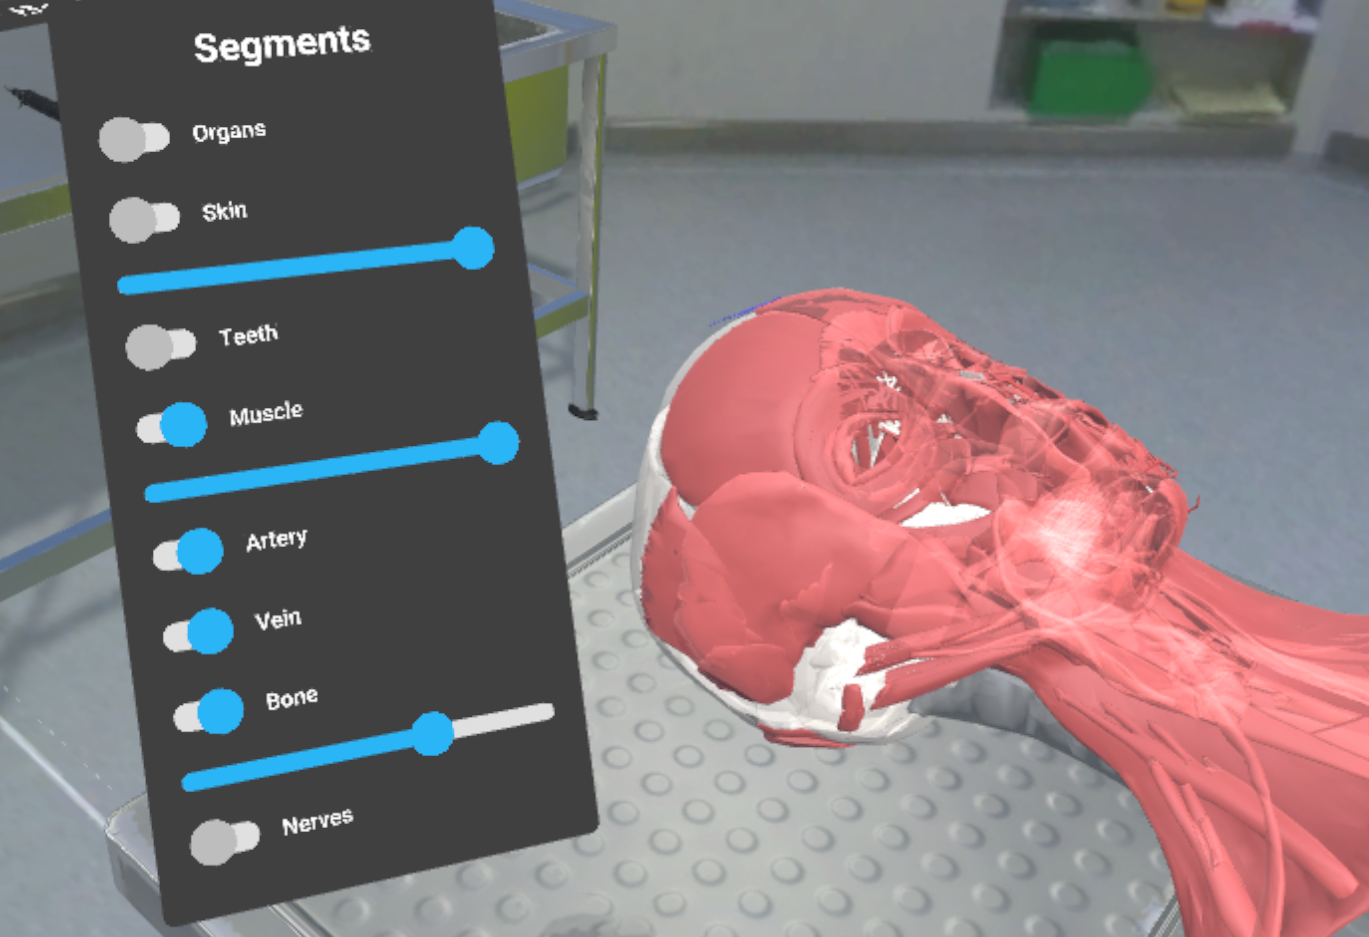
\includegraphics[width=0.95\linewidth]{images/implementation/features/visualization/segments_1.png}
  \end{minipage}%
  \begin{minipage}{.5\textwidth}
    \centering
    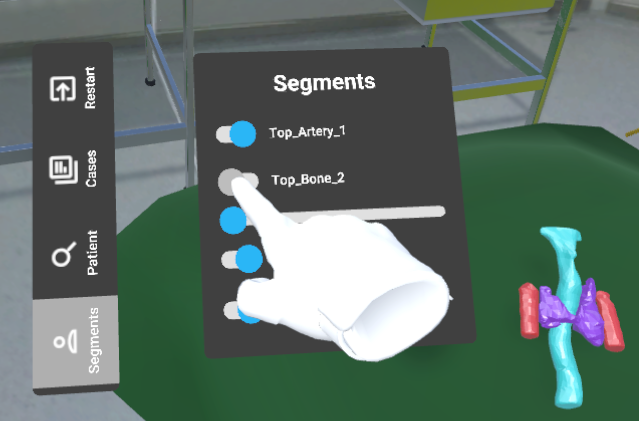
\includegraphics[width=0.915\linewidth]{images/implementation/features/visualization/segments_2.png}
  \end{minipage}
  \caption{\label{fig::Segmentation}Visualization - Segmentation}
\end{figure}

In Figure \ref{fig::Segmentation}, the process of activating and deactivating specific segments is described.
Users can also decide to adjust the transparency of segments as desired.
Additionally, the whole virtual patient can be scaled and up and down via their respective button.
Also, the user can reset the scale, position and rotation of the patients 3D model at any time to their defaults.

\begin{figure}[ht!]
  \centering
  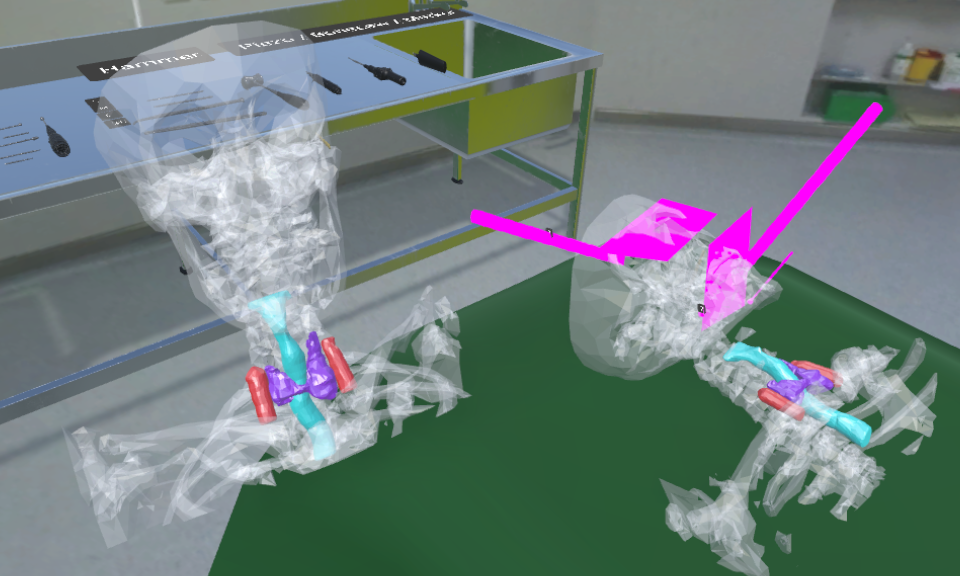
\includegraphics[width=\linewidth]{images/implementation/features/visualization/project_copy.png}
  \caption{\label{fig::ProjectCopy} Project a Copy of the Initial Patient for Comparison}
\end{figure}

Additionally, the user can at any time spawn a copy of the default patient, without any procedure steps, for comparison (Figure \ref{fig::ProjectCopy}).

The main model of the patient can also be exploded as depicted in Figure \ref{fig::Segmentation}.
Here, segments are exploded in a circular to allow for a closer look at each individual segment of the patient.

\begin{figure}[ht!]
    \centering
    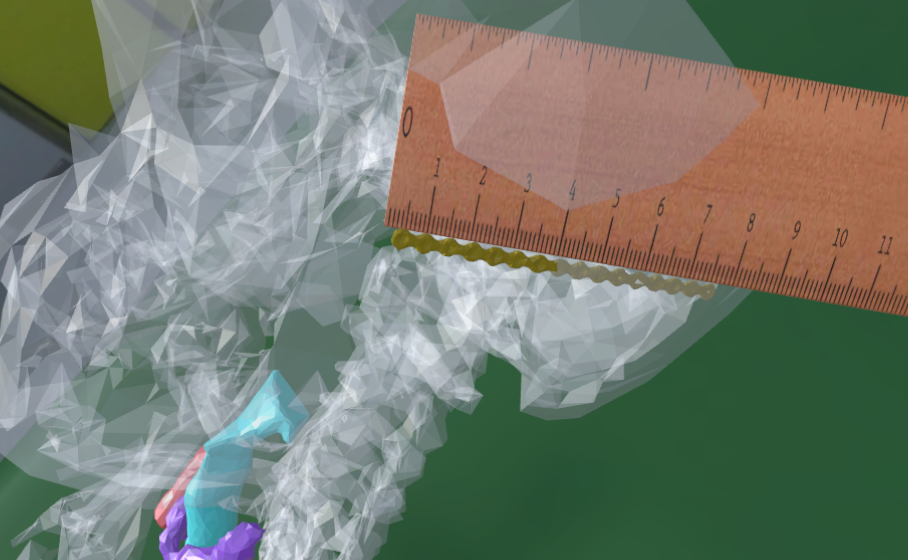
\includegraphics[width=\linewidth]{images/implementation/features/visualization/ruler.png}
    \caption{\label{fig::FeatureRuler} Ruler for Checking distances}
\end{figure}

In the virtual operating room, a ruler can be used to measure distances, but more importantly relative distances in the patients morphology.
The ruler can simply be picked up via a grab gesture and used in the same way a surgeon uses it in the medical field.